%# -*- coding: utf-8-unix -*-
%%==================================================
\tikzset{every picture/.style={line width=0.75pt}} %set default line width to 0.75pt    

\chapter{力学}

\label{s_hx}
\section{换系}

\section{惯性力}

\label{s_yhzl}
\section{约化质量}

\section{质心系}

\subsection{质心与质心系}

若一个系统由多个质点组成,其整个系统的质量可等效集中于一点,即质心。

\label{zxdy}
\begin{theo}{质心定义}{}
若各质点质量与坐标分别为$m_1$、$(x_1,y_1)$,$m_2$、$(x_2,y_2)$……$m_n$、$(x_n,y_n)$,则质心位置为
$$x_c = \frac{\sum m_i x_i}{\sum m_i} \quad y_c = \frac{\sum m_i y_i}{\sum m_i}$$
\end{theo}

质心在物理中有很多应用,如如果重力场是匀强场($g$为定值),则重心与质心重合,因此,重力势能的变化可以利用质心来计算。

\begin{ep}{练习题}{}
\begin{center}
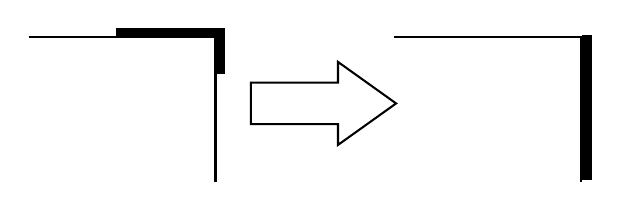
\begin{tikzpicture}[x=0.75pt,y=0.75pt,yscale=-1,xscale=1]
%uncomment if require: \path (0,300); %set diagram left start at 0, and has height of 300

%Straight Lines [id:da9215028484159156] 
\draw    (160,110) -- (250,110) -- (250,180) ;
%Straight Lines [id:da4977009583781107] 
\draw [line width=3.75]    (202,108) -- (252,108) -- (252,128) ;
%Straight Lines [id:da05737004026783943] 
\draw    (336,110) -- (426,110) -- (426,180) ;
%Right Arrow [id:dp10160418920196324] 
\draw   (267,132) -- (309,132) -- (309,122) -- (337,142) -- (309,162) -- (309,152) -- (267,152) -- cycle ;
%Straight Lines [id:da0051989052324770135] 
\draw [line width=3.75]    (429,109) -- (429,179) ;
\end{tikzpicture}
\end{center}
如图所示,有一总质量为$M=1kg$,总长度为$L=1m$的重绳,开始时有$L_0 = 0.2m$悬挂于桌边,后由于微扰重绳向右滑落,当重绳左端到达桌沿时,求重绳速度。(忽略重绳与桌面摩擦,桌子足够高以致重绳左端到达桌沿时右端未触地)
~\\

\begin{minipage}[b]{0.65\linewidth}
选取桌面为零势能面,向下为正方向,线密度$\lambda = \frac{M}{L} = 1kg/s$。初态质心位置为$y_c = \frac{\lambda L_0}{2} = 0.1J$,末态质心位置为$y_c^{\prime} = \frac{\lambda L}{2} = 0.5J$,由能量守恒可得$\frac{1}{2} M v^2 = Mg(y_c^{\prime}-y_c)$,解得$v = \frac{2\sqrt{5}}{5}$
\end{minipage}
\hfill
\begin{minipage}[b]{0.35\linewidth}
\begin{center}
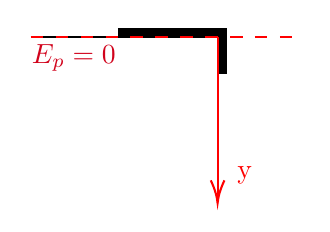
\begin{tikzpicture}[x=0.75pt,y=0.75pt,yscale=-1,xscale=1]
%uncomment if require: \path (0,300); %set diagram left start at 0, and has height of 300

%Straight Lines [id:da9215028484159156] 
\draw    (160,110) -- (250,110) -- (250,180) ;
%Straight Lines [id:da4977009583781107] 
\draw [line width=3.75]    (202,108) -- (252,108) -- (252,128) ;
%Straight Lines [id:da23325832635314958] 
\draw [color={rgb, 255:red, 255; green, 0; blue, 0 }  ,draw opacity=1 ]   (250,110) -- (250,188) ;
\draw [shift={(250,190)}, rotate = 270] [color={rgb, 255:red, 255; green, 0; blue, 0 }  ,draw opacity=1 ][line width=0.75]    (10.93,-3.29) .. controls (6.95,-1.4) and (3.31,-0.3) .. (0,0) .. controls (3.31,0.3) and (6.95,1.4) .. (10.93,3.29)   ;
%Straight Lines [id:da8953033878619383] 
\draw [color={rgb, 255:red, 255; green, 0; blue, 0 }  ,draw opacity=1 ] [dash pattern={on 4.5pt off 4.5pt}]  (160,110) -- (290,110) ;

% Text Node
\draw (258,171) node [anchor=north west][inner sep=0.75pt]  [color={rgb, 255:red, 255; green, 0; blue, 0 }  ,opacity=1 ] [align=left] {y};
% Text Node
\draw (159,112) node [anchor=north west][inner sep=0.75pt]   [align=left] {$\displaystyle \textcolor[rgb]{0.82,0.01,0.11}{E_{p} =0}$};
\end{tikzpicture}
\end{center}
\end{minipage}
\end{ep}

\subsection{质心与系统总动量}
质心还可用于求系统的总动量。由前文质心定义\eqref{zxdy},两端求导,得到
\begin{subequations}
\begin{align*}
M v_{cx} &= M \frac{d x_c}{dt} = \sum m_i \frac{d x_c}{dt} = \sum m_i v_{ix} \\
M v_{cy} &= M \frac{d y_c}{dt} = \sum m_i \frac{d y_c}{dt} = \sum m_i v_{iy}
\end{align*}
\end{subequations}

综上,有如下定理

\label{zxyxtzdl}
\begin{theo}{质心与系统总动量}{}
一个系统的总动量等于系统总质量乘上质心速度,即$\vec{p} = m_{tot} \vec{v}$($m_{tot}$为系统总质量\footnote{这里下标tot为total缩写})
\end{theo}

利用该定理,我们可以得到一个多星系统的很有用的结论
~\\

\begin{minipage}[b]{0.35\linewidth}
\begin{center}
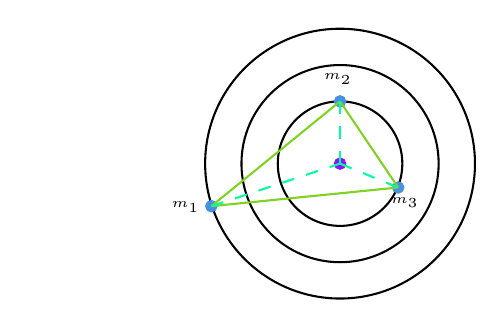
\begin{tikzpicture}[x=0.75pt,y=0.75pt,yscale=-1,xscale=1]
%uncomment if require: \path (0,300); %set diagram left start at 0, and has height of 300

%Straight Lines [id:da7411767697224816] 
\draw    (100,102) ;
%Shape: Circle [id:dp9490684003061072] 
\draw   (220,140) .. controls (220,123.43) and (233.43,110) .. (250,110) .. controls (266.57,110) and (280,123.43) .. (280,140) .. controls (280,156.57) and (266.57,170) .. (250,170) .. controls (233.43,170) and (220,156.57) .. (220,140) -- cycle ;
%Shape: Circle [id:dp9814343956363334] 
\draw   (202.5,140) .. controls (202.5,113.77) and (223.77,92.5) .. (250,92.5) .. controls (276.23,92.5) and (297.5,113.77) .. (297.5,140) .. controls (297.5,166.23) and (276.23,187.5) .. (250,187.5) .. controls (223.77,187.5) and (202.5,166.23) .. (202.5,140) -- cycle ;
%Shape: Circle [id:dp685701971148887] 
\draw   (185,140) .. controls (185,104.1) and (214.1,75) .. (250,75) .. controls (285.9,75) and (315,104.1) .. (315,140) .. controls (315,175.9) and (285.9,205) .. (250,205) .. controls (214.1,205) and (185,175.9) .. (185,140) -- cycle ;
%Shape: Circle [id:dp08570959225680785] 
\draw  [color={rgb, 255:red, 144; green, 19; blue, 254 }  ,draw opacity=1 ][fill={rgb, 255:red, 144; green, 19; blue, 254 }  ,fill opacity=1 ] (252.5,140) .. controls (252.5,138.62) and (251.38,137.5) .. (250,137.5) .. controls (248.62,137.5) and (247.5,138.62) .. (247.5,140) .. controls (247.5,141.38) and (248.62,142.5) .. (250,142.5) .. controls (251.38,142.5) and (252.5,141.38) .. (252.5,140) -- cycle ;
%Shape: Circle [id:dp47337912414359584] 
\draw  [color={rgb, 255:red, 74; green, 144; blue, 226 }  ,draw opacity=1 ][fill={rgb, 255:red, 74; green, 144; blue, 226 }  ,fill opacity=1 ] (280.5,151.5) .. controls (280.5,150.12) and (279.38,149) .. (278,149) .. controls (276.62,149) and (275.5,150.12) .. (275.5,151.5) .. controls (275.5,152.88) and (276.62,154) .. (278,154) .. controls (279.38,154) and (280.5,152.88) .. (280.5,151.5) -- cycle ;
%Shape: Circle [id:dp40050388744279153] 
\draw  [color={rgb, 255:red, 74; green, 144; blue, 226 }  ,draw opacity=1 ][fill={rgb, 255:red, 74; green, 144; blue, 226 }  ,fill opacity=1 ] (252.5,110) .. controls (252.5,108.62) and (251.38,107.5) .. (250,107.5) .. controls (248.62,107.5) and (247.5,108.62) .. (247.5,110) .. controls (247.5,111.38) and (248.62,112.5) .. (250,112.5) .. controls (251.38,112.5) and (252.5,111.38) .. (252.5,110) -- cycle ;
%Shape: Circle [id:dp5599587744609031] 
\draw  [color={rgb, 255:red, 74; green, 144; blue, 226 }  ,draw opacity=1 ][fill={rgb, 255:red, 74; green, 144; blue, 226 }  ,fill opacity=1 ] (190.5,160.5) .. controls (190.5,159.12) and (189.38,158) .. (188,158) .. controls (186.62,158) and (185.5,159.12) .. (185.5,160.5) .. controls (185.5,161.88) and (186.62,163) .. (188,163) .. controls (189.38,163) and (190.5,161.88) .. (190.5,160.5) -- cycle ;
%Straight Lines [id:da384151252822579] 
\draw [color={rgb, 255:red, 126; green, 211; blue, 33 }  ,draw opacity=1 ]   (188,160.5) -- (278,151.5) ;
%Straight Lines [id:da24848451118665693] 
\draw [color={rgb, 255:red, 126; green, 211; blue, 33 }  ,draw opacity=1 ]   (188,160.5) -- (250,110) ;
%Straight Lines [id:da8234484439529937] 
\draw [color={rgb, 255:red, 126; green, 211; blue, 33 }  ,draw opacity=1 ]   (250,110) -- (278,151.5) ;
%Straight Lines [id:da4853630824410369] 
\draw [color={rgb, 255:red, 0; green, 255; blue, 165 }  ,draw opacity=1 ] [dash pattern={on 4.5pt off 4.5pt}]  (188,160.5) -- (250,140) ;
%Straight Lines [id:da04897594598262511] 
\draw [color={rgb, 255:red, 0; green, 255; blue, 165 }  ,draw opacity=1 ] [dash pattern={on 4.5pt off 4.5pt}]  (250,140) -- (278,151.5) ;
%Straight Lines [id:da013808732174074745] 
\draw [color={rgb, 255:red, 0; green, 255; blue, 165 }  ,draw opacity=1 ] [dash pattern={on 4.5pt off 4.5pt}]  (250,110) -- (250,140) ;

% Text Node
\draw (167.33,157) node [anchor=north west][inner sep=0.75pt]  [font=\tiny] [align=left] {$\displaystyle m_{1}$};
% Text Node
\draw (240.67,95.33) node [anchor=north west][inner sep=0.75pt]  [font=\tiny] [align=left] {$ $$\displaystyle m_{2}$};
% Text Node
\draw (273,155) node [anchor=north west][inner sep=0.75pt]  [font=\tiny] [align=left] {$\displaystyle m_{3}$};


\end{tikzpicture}

\end{center}

\end{minipage}
\hfill
\begin{minipage}[b]{0.55\linewidth}
\begin{theo}{相对静止多星系统的公共圆心}{}
对于一个多星系统,若各星之间相对静止,则该多星系统的公共圆心为该系统质心
\end{theo}
\end{minipage}
~\\

对于如上定理,可用反证法证明,证明如下:

假定多星系统公共圆心不在质心处,则质心必定绕公共圆心做匀速圆周运动,那么根据之前的定理系统,系统总动量等于系统总质量乘上质心速度,故系统总质量方向将一直在变化。而该多星系统整体不受外力,因此系统总动量必须守恒,这与之前假设不符,故先前假设不成立,QED\footnote{QED为拉丁文quod erat demonstrandum的缩写,意为“证毕”}。

在大多数解析中,此类题目采取的思路是作最一般的位置假设,然后列方程计算。此定理跳过了繁琐的的方程求解,并令解题有了更强的方向性,不至于“无头苍蝇”。

\begin{mk}{易错提醒}{}
在此特别提醒,\textbf{万有引力计算绝不可以用质心},因为万有引力与距离关系不是一次函数关系,而是平方反比关系。\textbf{多星系统中某个天体向心力只能分别用万有引力定律计算相互之间引力,再利用平行四边形法则合成力}。
\end{mk}

\begin{ep}{练习题}{}
由三颗星体构成的系统,忽略其他星体对它们的作用,存在着种运动形式:三颗星体在相互之间的万有引力作用下,分别位于等边三角形的三个顶点上,绕某一共同的圆心$O$在三角形所在的平面内做相同角速度的圆周运动。若A星体的质量为$2m$,B、C两星体的质量均为$m$,三角形的边长为$a$,求:

\begin{enumerate}[label=(\arabic*)]
  \item A星体所受合力大小$F_A$;
  \item B星体所受合力大小$F_B$;
  \item C星体轨道半径$R_C$;
  \item 三星体做圆周运动周期$T$。
\end{enumerate}
~\\

\begin{minipage}[b]{0.65\linewidth}
(1) 如图所示,由万有引力公式$F_{BA}=F_{CA}=\frac{2 G m^2}{a^2}$,合力$F_A = \sqrt{3} F_{BA} = \frac{2\sqrt{3} G m^2}{a^2}$
~\\

(2) A对B引力$F_{AB}=\frac{2 G m^2}{a^2}$,C对B引力$F_{CB}=\frac{G m^2}{a^2}$,在矢量三角形中使用余弦定理,得
$$F_B = \sqrt{F_{AB}^2+F_{CB}^2-2F_{AB} \cdot F_{CB} \cos{120^{\circ}}}=\frac{\sqrt{7}G m^2}{a^2}$$
\end{minipage}
\hfill
\begin{minipage}[b]{0.35\linewidth}
\begin{center}
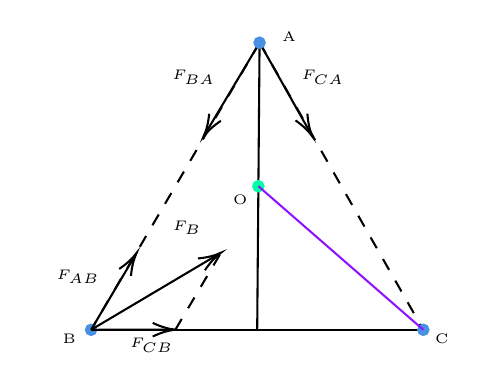
\begin{tikzpicture}[x=0.75pt,y=0.75pt,yscale=-1,xscale=1]
%uncomment if require: \path (0,300); %set diagram left start at 0, and has height of 300

%Straight Lines [id:da7411767697224816] 
\draw    (100,102) ;
%Straight Lines [id:da35334013949437937] 
\draw    (130.05,191.39) -- (290.12,191.39) ;
%Straight Lines [id:da8337888464734036] 
\draw    (211.23,53.05) -- (210.08,191.39) ;
%Straight Lines [id:da37892752623854364] 
\draw    (211.23,53.05) -- (185.19,96.68) ;
\draw [shift={(184.17,98.4)}, rotate = 300.82] [color={rgb, 255:red, 0; green, 0; blue, 0 }  ][line width=0.75]    (10.93,-3.29) .. controls (6.95,-1.4) and (3.31,-0.3) .. (0,0) .. controls (3.31,0.3) and (6.95,1.4) .. (10.93,3.29)   ;
%Straight Lines [id:da23461063513640812] 
\draw  [dash pattern={on 4.5pt off 4.5pt}]  (211.23,53.05) -- (130.05,191.39) ;
%Straight Lines [id:da4163775253760995] 
\draw  [dash pattern={on 4.5pt off 4.5pt}]  (211.23,53.05) -- (290.12,191.39) ;
%Straight Lines [id:da14314395431520932] 
\draw    (211.23,53.05) -- (235.78,96.66) ;
\draw [shift={(236.76,98.4)}, rotate = 240.62] [color={rgb, 255:red, 0; green, 0; blue, 0 }  ][line width=0.75]    (10.93,-3.29) .. controls (6.95,-1.4) and (3.31,-0.3) .. (0,0) .. controls (3.31,0.3) and (6.95,1.4) .. (10.93,3.29)   ;
%Shape: Circle [id:dp27435800391771203] 
\draw  [color={rgb, 255:red, 74; green, 144; blue, 226 }  ,draw opacity=1 ][fill={rgb, 255:red, 74; green, 144; blue, 226 }  ,fill opacity=1 ] (213.73,53.05) .. controls (213.73,51.67) and (212.61,50.55) .. (211.23,50.55) .. controls (209.85,50.55) and (208.73,51.67) .. (208.73,53.05) .. controls (208.73,54.43) and (209.85,55.55) .. (211.23,55.55) .. controls (212.61,55.55) and (213.73,54.43) .. (213.73,53.05) -- cycle ;
%Shape: Circle [id:dp355067680258665] 
\draw  [color={rgb, 255:red, 74; green, 144; blue, 226 }  ,draw opacity=1 ][fill={rgb, 255:red, 74; green, 144; blue, 226 }  ,fill opacity=1 ] (132.55,191.39) .. controls (132.55,190.01) and (131.43,188.89) .. (130.05,188.89) .. controls (128.67,188.89) and (127.55,190.01) .. (127.55,191.39) .. controls (127.55,192.77) and (128.67,193.89) .. (130.05,193.89) .. controls (131.43,193.89) and (132.55,192.77) .. (132.55,191.39) -- cycle ;
%Shape: Circle [id:dp8731378911211072] 
\draw  [color={rgb, 255:red, 74; green, 144; blue, 226 }  ,draw opacity=1 ][fill={rgb, 255:red, 74; green, 144; blue, 226 }  ,fill opacity=1 ] (292.62,191.39) .. controls (292.62,190.01) and (291.5,188.89) .. (290.12,188.89) .. controls (288.74,188.89) and (287.62,190.01) .. (287.62,191.39) .. controls (287.62,192.77) and (288.74,193.89) .. (290.12,193.89) .. controls (291.5,193.89) and (292.62,192.77) .. (292.62,191.39) -- cycle ;
%Shape: Circle [id:dp08553461642771443] 
\draw  [color={rgb, 255:red, 0; green, 255; blue, 165 }  ,draw opacity=1 ][fill={rgb, 255:red, 0; green, 255; blue, 165 }  ,fill opacity=1 ] (213.15,122.22) .. controls (213.15,120.84) and (212.04,119.72) .. (210.65,119.72) .. controls (209.27,119.72) and (208.15,120.84) .. (208.15,122.22) .. controls (208.15,123.6) and (209.27,124.72) .. (210.65,124.72) .. controls (212.04,124.72) and (213.15,123.6) .. (213.15,122.22) -- cycle ;
%Straight Lines [id:da7509716289501367] 
\draw [color={rgb, 255:red, 144; green, 19; blue, 254 }  ,draw opacity=1 ]   (210.65,122.22) -- (290.12,191.39) ;
%Straight Lines [id:da6715627766530636] 
\draw    (130.05,191.39) -- (168.67,191.34) ;
\draw [shift={(170.67,191.33)}, rotate = 179.92] [color={rgb, 255:red, 0; green, 0; blue, 0 }  ][line width=0.75]    (10.93,-3.29) .. controls (6.95,-1.4) and (3.31,-0.3) .. (0,0) .. controls (3.31,0.3) and (6.95,1.4) .. (10.93,3.29)   ;
%Straight Lines [id:da8234752419975047] 
\draw    (130.05,191.39) -- (150.98,156.05) ;
\draw [shift={(152,154.33)}, rotate = 120.64] [color={rgb, 255:red, 0; green, 0; blue, 0 }  ][line width=0.75]    (10.93,-3.29) .. controls (6.95,-1.4) and (3.31,-0.3) .. (0,0) .. controls (3.31,0.3) and (6.95,1.4) .. (10.93,3.29)   ;
%Straight Lines [id:da371469419005255] 
\draw  [dash pattern={on 4.5pt off 4.5pt}]  (170.67,191.33) -- (192.62,154.27) ;
%Straight Lines [id:da13561111516549063] 
\draw    (130.05,191.39) -- (190.9,155.29) ;
\draw [shift={(192.62,154.27)}, rotate = 149.32] [color={rgb, 255:red, 0; green, 0; blue, 0 }  ][line width=0.75]    (10.93,-3.29) .. controls (6.95,-1.4) and (3.31,-0.3) .. (0,0) .. controls (3.31,0.3) and (6.95,1.4) .. (10.93,3.29)   ;

% Text Node
\draw (220.67,46.33) node [anchor=north west][inner sep=0.75pt]  [font=\tiny] [align=left] {A};
% Text Node
\draw (115,192) node [anchor=north west][inner sep=0.75pt]  [font=\tiny] [align=left] {B};
% Text Node
\draw (294.33,192) node [anchor=north west][inner sep=0.75pt]  [font=\tiny] [align=left] {C};
% Text Node
\draw (197,125) node [anchor=north west][inner sep=0.75pt]  [font=\tiny] [align=left] {O};
% Text Node
\draw (167.67,64.67) node [anchor=north west][inner sep=0.75pt]  [font=\tiny] [align=left] {$\displaystyle F_{BA}$};
% Text Node
\draw (230,64.67) node [anchor=north west][inner sep=0.75pt]  [font=\tiny] [align=left] {$\displaystyle F_{CA}$};
% Text Node
\draw (112,161) node [anchor=north west][inner sep=0.75pt]  [font=\tiny] [align=left] {$\displaystyle F_{AB}$};
% Text Node
\draw (147.33,194) node [anchor=north west][inner sep=0.75pt]  [font=\tiny] [align=left] {$\displaystyle F_{CB}$};
% Text Node
\draw (168,137.33) node [anchor=north west][inner sep=0.75pt]  [font=\tiny] [align=left] {$\displaystyle F_{B}$};
\end{tikzpicture}

\end{center}
\end{minipage}
~\\

(3) B、C质心在BC中点,等效质量为$2m$,故三星系统质心在A与BC中点的连线的中点(O点)上,故由几何关系
$$R_C^2 = (\frac{1}{2} \cdot \frac{\sqrt{3}}{2} a)^2+(\frac{a}{2})^2$$
解得$R_C = \frac{\sqrt{7}}{4} a$
~\\

(4) 由对称性
$$F_C = F_B = \frac{\sqrt{7}G m^2}{a^2} = m \omega ^2 R_C$$
故$T=\frac{2 \pi}{\omega}=\pi \sqrt{\frac{a^3}{G m}}$

\end{ep}

若我们将系统看为整体,由动量定理,当且仅当这个整体受到外力时,系统总动量改变,因此有

\begin{theo}{系统动量定理}{}
对于一个质点系而言,只有合外力才会导致系统总动量发生变化,内力不影响系统总动量。
\end{theo}

\subsection{质心系}

若我们选取系统的质心为参考点建立参考系,则我们称此参考系为\textbf{质心系}(记为CM系\footnote{CM为Center of Mass的缩写,意为“质心”})。

\label{zxxsd}
\begin{theo}{质心系速度}{}
根据前文质心定义\eqref{zxdy},对其两端对时间求导,可得

$$v_{cx} = \frac{\sum m_i v_{ix}}{\sum m_i} \quad v_{cy} = \frac{\sum m_i v_{iy}}{\sum m_i}$$
\end{theo}

在质心系中,有如下性质

\begin{theo}{质心系系统动量}{}
在质心系中,质心速度为$0$,则根据定理\eqref{zxyxtzdl},系统总动量为$0$,即\textbf{质心系下系统的总动量为零}。写成矢量式为

\label{e_zxxdl}
\begin{subequations}
\begin{align*}
\sum m_i \cdot \vec{v_{ci}} = 0
\end{align*}
\end{subequations}

其中$\vec{v_{ci}}$为第$i$个物体在质心系中速度。
\end{theo}

\subsection{质心系动能定理}

如果系统只做平动,系统中质点各个部分的速度完全相同,则物体可视为质点,动能当然可以由质心速度来计算。但当系统中质点有相对质心的运动时,则系统动能应由柯尼希(König)定理计算

\begin{theo}{柯尼希定理}{}
若系统中有$n$个质点,质点质量和相对质心速度分别为$m_1$、$v_{c1}$,$m_2$、$v_{c2}$……$m_n$、$v_{cn}$,则体系总动能为

$$E_{tot}=\frac{1}{2} m_{tot} v_c^2 + \sum \frac{1}{2} m_i v_{ci}^2$$

其中$m_{tot} = \sum m_i$为系统总质量,$v_c$为质心速度。记$\frac{1}{2} m_{tot} v_c^2$为质心动能,$\sum \frac{1}{2} m_i v_{ci}^2$为相对质心动能。即\textbf{系统总动能等于质心动能加上其他质点相对质心动能}。
\end{theo}

\begin{mk}{易错提醒}{}
根据柯尼希定理,由于系统总动能包含相对质心的动能这一项,故\textbf{不可以用质心速度变化来计算动能的变化量}。
\end{mk}

柯尼希定理证明如下:

在地面参考系中,质心速度为$\vec{v_c}$,第$i$个相对质心速度为$\vec{v_{ci}}$,根据前文\eqref{s_hx},第$i$个质点相对地面速度为

$$\vec{v_i} = \vec{v_c} + \vec{v_{ci}}$$

则总动能

\begin{subequations}
\begin{align*}
E_{tot} &= \sum \frac{1}{2} m_i \vec{v_i}^2 \\
&= \sum \frac{1}{2} m_i \vec{v_i}^2 + \sum \frac{1}{2} m_i \vec{v_{ci}}^2 + \vec{v_i} \cdot \sum m_i \vec{v_{ci}} \\
&= \frac{1}{2} m_{tot} v_c^2 + \sum \frac{1}{2} m_i v_{ci}^2
\end{align*}
\end{subequations}

证毕,QED。 

我们可以用此定理很快地得到完全非弹性碰撞损失能量公式。若两球发生完全非弹性碰撞,记两球质量和初速分别为$m_1$、$v_1$,$m_2$、$v_2$。则根据质心系速度\eqref{zxxsd},可得

$$v_c = \frac{m_1 v_1 + m_2 v_2}{m_1+m_2}$$

两球相对质心速度分别为

$$v_{c1} = v_1 - v_c \quad v_{c2} = v_2 - v_c$$

由于系统动量守恒,故系统动量保持不变,质心动量保持不变,根据$p^2 = 2 m E_k$知质心动能保持不变。那么当相对质心速度均为$0$时,相对质心动能为$0$,此时系统总动能最小,两球共速(均为质心速度),能量损失最大。那么此时损失的能量

\begin{subequations}
\begin{align*}
\Delta E &= \frac{1}{2} m_1 v_{c1}^2 + \frac{1}{2} m_2 v_{c2}^2 \\
&= \frac{1}{2} \mu (v_2 - v_1)^2 \\
&= \frac{1}{2} \mu v_{in}^2
\end{align*}
\end{subequations}

即完全非弹性碰撞的能量损失公式。故有如下定理

\begin{theo}{碰撞中能量损失最值}{}
在两物体碰撞中,当碰撞为完全非弹性碰撞时,系统能量损失最大,为

$$\Delta E_{max} = \frac{1}{2} \mu v_{in}^2$$

其中$\mu$为约化质量\eqref{s_yhzl},$v_{in}$为两球相对接近速度。
\end{theo}

\section{等效碰撞}

\subsection{等效完全非弹性碰撞}

\subsection{等效完全弹性碰撞}

\section{恢复系数}

\subsection{定义与基本性质}

\begin{center}
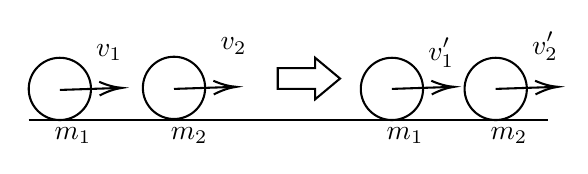
\begin{tikzpicture}[x=0.75pt,y=0.75pt,yscale=-1,xscale=1]
%uncomment if require: \path (0,300); %set diagram left start at 0, and has height of 300
%Straight Lines [id:da5712311460225725] 
\draw    (100,110) -- (350,110) ;
%Shape: Circle [id:dp501626887330255] 
\draw   (100,95) .. controls (100,86.72) and (106.72,80) .. (115,80) .. controls (123.28,80) and (130,86.72) .. (130,95) .. controls (130,103.28) and (123.28,110) .. (115,110) .. controls (106.72,110) and (100,103.28) .. (100,95) -- cycle ;
%Shape: Circle [id:dp8027430983175681] 
\draw   (155,94.5) .. controls (155,86.22) and (161.72,79.5) .. (170,79.5) .. controls (178.28,79.5) and (185,86.22) .. (185,94.5) .. controls (185,102.78) and (178.28,109.5) .. (170,109.5) .. controls (161.72,109.5) and (155,102.78) .. (155,94.5) -- cycle ;
%Shape: Circle [id:dp23940754387998542] 
\draw   (310,95) .. controls (310,86.72) and (316.72,80) .. (325,80) .. controls (333.28,80) and (340,86.72) .. (340,95) .. controls (340,103.28) and (333.28,110) .. (325,110) .. controls (316.72,110) and (310,103.28) .. (310,95) -- cycle ;
%Shape: Circle [id:dp9006459635140887] 
\draw   (260,95) .. controls (260,86.72) and (266.72,80) .. (275,80) .. controls (283.28,80) and (290,86.72) .. (290,95) .. controls (290,103.28) and (283.28,110) .. (275,110) .. controls (266.72,110) and (260,103.28) .. (260,95) -- cycle ;
%Right Arrow [id:dp7037165842832618] 
\draw   (220,85) -- (238,85) -- (238,80) -- (250,90) -- (238,100) -- (238,95) -- (220,95) -- cycle ;
%Straight Lines [id:da3133909490523399] 
\draw    (115,95.5) -- (143,94.57) ;
\draw [shift={(145,94.5)}, rotate = 178.09] [color={rgb, 255:red, 0; green, 0; blue, 0 }  ][line width=0.75]    (10.93,-3.29) .. controls (6.95,-1.4) and (3.31,-0.3) .. (0,0) .. controls (3.31,0.3) and (6.95,1.4) .. (10.93,3.29)   ;
%Straight Lines [id:da03685629638481602] 
\draw    (170,95) -- (198,94.07) ;
\draw [shift={(200,94)}, rotate = 178.09] [color={rgb, 255:red, 0; green, 0; blue, 0 }  ][line width=0.75]    (10.93,-3.29) .. controls (6.95,-1.4) and (3.31,-0.3) .. (0,0) .. controls (3.31,0.3) and (6.95,1.4) .. (10.93,3.29)   ;
%Straight Lines [id:da15780397999919527] 
\draw    (275,95) -- (303,94.07) ;
\draw [shift={(305,94)}, rotate = 178.09] [color={rgb, 255:red, 0; green, 0; blue, 0 }  ][line width=0.75]    (10.93,-3.29) .. controls (6.95,-1.4) and (3.31,-0.3) .. (0,0) .. controls (3.31,0.3) and (6.95,1.4) .. (10.93,3.29)   ;
%Straight Lines [id:da1252447585559464] 
\draw    (325,95) -- (353,94.07) ;
\draw [shift={(355,94)}, rotate = 178.09] [color={rgb, 255:red, 0; green, 0; blue, 0 }  ][line width=0.75]    (10.93,-3.29) .. controls (6.95,-1.4) and (3.31,-0.3) .. (0,0) .. controls (3.31,0.3) and (6.95,1.4) .. (10.93,3.29)   ;

% Text Node
\draw (111,112) node [anchor=north west][inner sep=0.75pt]   [align=left] {$\displaystyle m_{1}$};
% Text Node
\draw (167,112) node [anchor=north west][inner sep=0.75pt]   [align=left] {$\displaystyle m_{2}$};
% Text Node
\draw (271,112) node [anchor=north west][inner sep=0.75pt]   [align=left] {$\displaystyle m_{1}$};
% Text Node
\draw (321,112) node [anchor=north west][inner sep=0.75pt]   [align=left] {$\displaystyle m_{2}$};
% Text Node
\draw (131,72) node [anchor=north west][inner sep=0.75pt]   [align=left] {$\displaystyle v_{1}$};
% Text Node
\draw (191,69) node [anchor=north west][inner sep=0.75pt]   [align=left] {$\displaystyle v_{2}$};
% Text Node
\draw (291,69) node [anchor=north west][inner sep=0.75pt]   [align=left] {$\displaystyle v_{1}^{\prime }$};
% Text Node
\draw (341,66) node [anchor=north west][inner sep=0.75pt]   [align=left] {$\displaystyle v_{2}^{\prime }$};
\end{tikzpicture}
\end{center}

对于两个物体的碰撞过程,假设两物体质量为$m_1$、$m_2$初态时速度分别为$v_1$、$v_2$(以向右为正方向),末态时为$v_1^{\prime}$、$v_2^{\prime}$

\begin{defi}{恢复系数}{}
记两个物体接近时相对速度(接近速度)$\Delta v_{in} = v_1-v_2$,分离时相对速度(分离速度)$\Delta v_{out} = v_2^{\prime}-v_1^{\prime}$,则定义恢复系数

$$e = \frac{\Delta v_{out}}{\Delta v_{in}}$$

即恢复系数等于接近速度除以分离速度。
\end{defi}

现我们探讨不同情况下的恢复系数:

对于完全非弹性碰撞,碰撞后两物体共速,即分离速度$\Delta v_{out} = 0$,故此时恢复系数$e=0$。

对于完全弹性碰撞,碰撞过程满足能量守恒和动量守恒,故有
\begin{subequations}
\begin{align}
\label{e_eq1}
\frac{1}{2} m_1 v_1^2 + \frac{1}{2} m_2 v_2^2 &= \frac{1}{2} m_1 {v_1^{\prime}}^2 + \frac{1}{2} m_2 {v_2^{\prime}}^2 \\
\label{e_eq2}
m_1 v_1 + m_2 v_2 &= m_1 v_1^{\prime} + m_2 v_2^{\prime} 
\end{align}
\end{subequations}

化简\eqref{e_eq1},移项,展开,得
\begin{subequations}
\begin{align}
\label{e_eq3}
m_1 (v_1 + v_1^{\prime})(v_1 - v_1^{\prime}) = m_2 (v_2 + v_2^{\prime})(v_2^{\prime} - v_2)  
\end{align}
\end{subequations}

将\eqref{e_eq3}除以移项后的\eqref{e_eq2},得$v_1 + v_1^{\prime} = v_2 + v_2^{\prime}$,即此时$e=1$。

\begin{theo}{完全弹性碰撞恢复系数}{}
在完全弹性碰撞中,恢复系数$e=1$,即\textbf{接近速度等于分离速度}
\end{theo}

对于非完全弹性碰撞,可以证明$0 < e <1$。

综上,我们可以用恢复系数表征不同碰撞类型,即:

\begin{itemize}
	\item 完全非弹性碰撞:$e = 0$
	\item 非完全弹性碰撞:$0 < e < 1$
	\item 完全弹性碰撞:$e = 1$
\end{itemize}

\subsection{恢复系数与能量关系}

从前文中我们可以得知,对于完全弹性碰撞,恢复系数$e=1$,$e=1$与能量守恒方程等价,可以借此简化完全弹性碰撞的公式推导。这一性质还可以在如下题目中将较复杂的能量计算转换为相对速度的计算,大大简化计算量。

\begin{ep}{练习题}{}
两球A、B在光滑水平线上沿同一直线,同一方向运动,$m_A = 1kg$,$m_B = 2kg$,$v_A = 6m/s$,$v_B = 2m/s$。当球A追上球B并发生碰撞后,两球A、B的速度可能是(取碰撞前两球运动方向为正)

A.$v_A^{\prime} = 5m/s$,$v_B^{\prime} = 2.5m/s$ \quad B.$v_A^{\prime} = 2m/s$,$v_B^{\prime} = 4m/s$

C.$v_A^{\prime} = -4m/s$,$v_B^{\prime} = 7m/s$ \quad D.$v_A^{\prime} = 7m/s$,$v_B^{\prime} = 1.5m/s$
~\\

对于上面四个选项,其动量均为$10kg \cdot m/s$,故只能从能量和两球速度判断。
由于碰撞后不可能出现球A、球B速度同向且A速度大于B速度的情况,故选项AD错误。由前文得知,分离速度不大于接近速度。接近速度$v_{in}=4m/s$,对于B,分离速度$v_{out} = 2m/s$;对于C,分离速度$v_{out} = 11m/s$,大于接近速度。故B对,C错。综上,选B。
\end{ep}

更进一步的,我们还可以求出$e$与体系因碰撞损失能量$\Delta E$的关系。

\begin{subequations}
\label{e_eq4}
\begin{align}
\Delta E &= \frac{1}{2} m_1 {v_1^{\prime}}^2 + \frac{1}{2} m_2 {v_2^{\prime}}^2 - \frac{1}{2} m_1 v_1^2 - \frac{1}{2} m_2 v_2^2 \\
0 &= m_1 v_1^{\prime} + m_2 v_2^{\prime} - m_1 v_1 - m_2 v_2 \\
e &= \frac{v_2^{\prime} - v_1^{\prime}}{v_1 - v_2}
\end{align}
\end{subequations}

联立\eqref{e_eq4},解得碰撞损失能量$\Delta E$与$e$的关系,如下

\begin{theo}{恢复系数与损失能量关系}{}
碰撞损失能量$\Delta E$与$e$满足如下关系
$$\Delta E = (1 - e^2) \cdot \frac{1}{2} \mu v_{in}^2 = (1 - e^2) \Delta E_{max}$$
其中$\mu$为前文中的约化质量\eqref{s_yhzl},接近速度$v_{in} = v_2 - v_1$
\end{theo}

\begin{mk}{思考}{}
此定理可以使用质心动能定理简便证明,试用质心动能定理证明该定理。
\end{mk}

这个定理可以应用在如下模型之中

\begin{ep}{自编题}{}
现有一质量为$M=0.9kg$的物体静止在光滑水平面上,一质量为$m=0.1kg$的子弹以速度$v=100m/s$打穿木块(忽略重力对子弹轨迹的偏移),穿出木块后木块速度为$v_M = 1m/s$,试求子弹穿出木块后子弹速度$v_m$及整个系统发热$Q$
~\\

先用动量守恒求出$v_m$:

$$m v = m v_m + M v_M$$

解的$v_m = 91m/s$。分离速度$v_{out} =  91 - 1 = 90m/s$,接近速度$v_{in} = 100m/s$因此$e = \frac{90}{100} = 0.9$,套用结论,得

$$\Delta E = (1 - 0.9^2) \cdot \frac{1}{2} \frac{0.9 \times 0.1}{0.9 + 0.1} \cdot 100^2 = 85.5J$$
\end{ep}

当然,以上模型还可以扩展到其他情况,如对于穿出过程中子弹得到加速,系统总机械能增加的情况,此时按照结论计算得到的$\Delta E$为负值,即损失了负数的能量,即其绝对值为系统总机械能增加值。但此情况出现很少,在此不再叙述。

\section{质心系反冲运动能量变化}